\section{Diseño}

En esta etapa de la metodología ágil, se debe elaborar un diseño que responda a las dificultades que los adultos mayores puedan experimentar probando juegos digitales. Encontrar el punto medio entre entretenimiento y aprendizaje, hacer una correcta integración de los elementos visuales y garantizar la legibilidad son algunos de los aspectos que se tratarán en este apartado.

\subsection{Diseño de la arquitectura}

La arquitectura completa de la skill se construirá sobre varias herramientas de \textit{Amazon Web Server} (AWS) que serán explicadas con mayor detalle en la sección 6. Estas se encuentran englobadas en \textit{AWS Serverless Platform}, una plataforma que permite la creación de skills sin necesidad de disponer de un servidor propio. 

Las tecnologías avanzadas de AWS más relevantes en el desarrollo de skills son: AWS Lambda, Amazon DynamoDB y Amazon S3.

\begin{figure}[H]
	\centering
	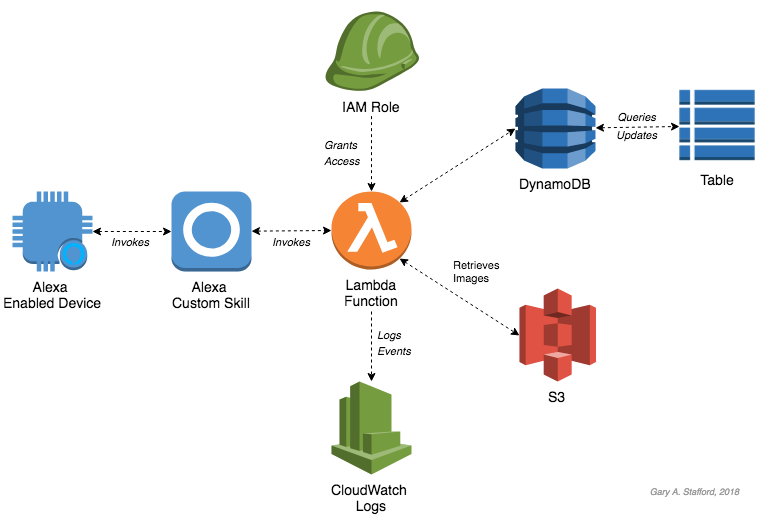
\includegraphics[width=0.98\textwidth]{imgs/arquitectura-skill.png}
	\caption{Arquitectura de una skill de Alexa con las tecnologías AWS \parencite{arquitecturaSkill}}
	\label{fig:arquitectura-skill}
\end{figure}


El proceso de creación de la habilidad para Alexa implica varios pasos clave \parencite{arquitecturaSkill}:
\begin{enumerate}
	\item Definir el modelo de interacción por voz; es decir, cómo los usuarios pueden invocar la skill con diversas intenciones mediante comandos de voz.
	\item Diseñar de la interfaz, solo en caso de que se vaya a desplegar en dispositivos con pantallas, para mejorar la experiencia de usuario al mostrar información visual complementaria al audio.
	\item Configurar las tablas en DynamoDB: para el almacenamiento persistente de información, usando una base de datos.
	\item Crear un bucket en S3 donde se alojarán las imágenes y vídeos requeridos para el paso 2.
	\item Programar la skill de Alexa, con funciones que permitan gestionar el flujo de conversación entre los usuarios y Alexa.
	\item Escribir la función Lambda, responsable de procesar las entradas del usuario y devolver las respuestas adecuadas, que peuden incluir datos almacenados en DynamoDB y en S3.
	\item Modificar el rol IAM predeterminado para que la función Lambda actualice la información de la base de datos según sea necesario.
	\item Desplegar y probar la skill para asegurarse de que funciona según lo esperado.
\end{enumerate}

Adicionalmente, para gestionar los elementos visuales que serán mostrados en la pantalla del dispositivo de Alexa, se tiene la siguiente arquitectura para el Lenguaje de Presentación de Alexa, comúnmente conocido como APL.

\begin{figure}[H]
	\centering
	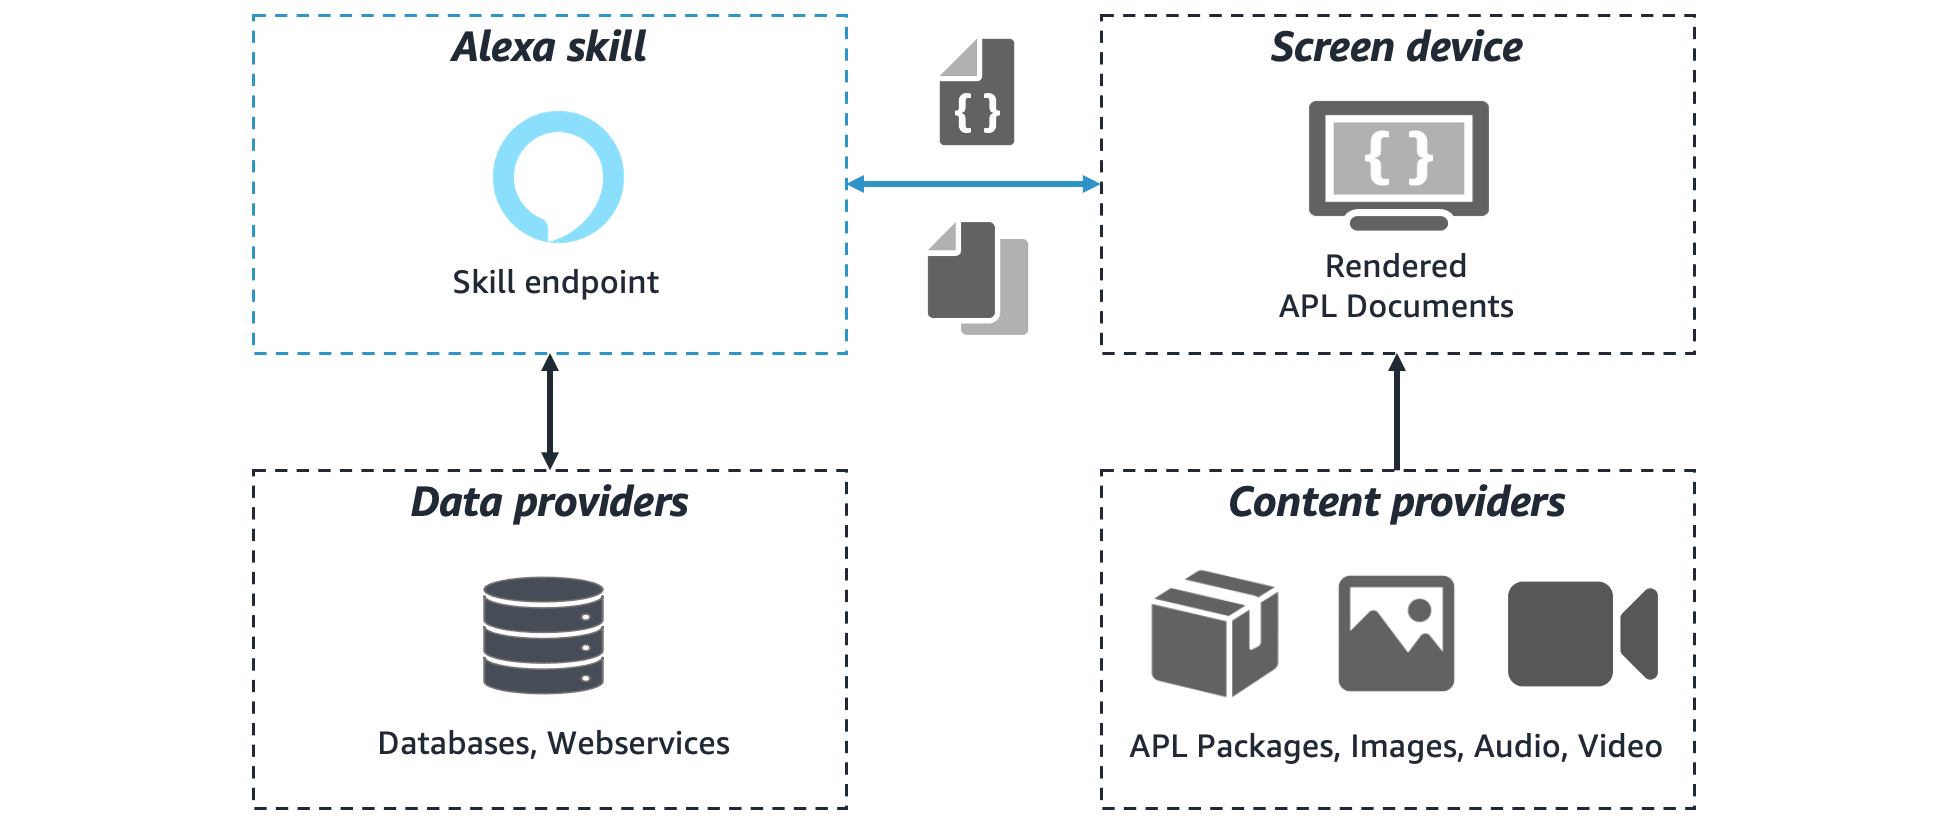
\includegraphics[width=0.98\textwidth]{imgs/arquitectura-apl.png}
	\caption{Arquitectura de una APL con los cuatro actores principales (\href{https://developer.amazon.com/en-US/docs/alexa/alexa-presentation-language/apl-bp-understand-apl-architecture.html}{Alexa Developer Documentation})}
\label{fig:arquitectura-apl}
\end{figure}

Los dos agentes esenciales son:
\begin{itemize}
	\item \textbf{La propia skill}: es la que inicia el proceso al enviar primero la plantilla del documento APL al dispositivo.
	\item \textbf{Los dispositivos con pantalla}: algunos dispositivos Alexa, como el Echo Show, son compatibles con este lenguaje de presentación y se encargan de mostrar por pantalla la plantilla APL. 
\end{itemize}

Los anteriores pueden ser complementados por agentes opcionales como: 
\begin{itemize}
	\item \textbf{Los proveedores de datos}: normalmente bases de datos como DynamoDB, almacenan de forma externa a la skill información relevante que puede ser consultada y/o modificada.
	\item \textbf{Los proveedores de contenido}: como Amazon S3, que incluyen archivos multimedia externos, que se almacenan públicamente en la red y son referenciados desde la skill mediante URLs. 
\end{itemize}

\subsection{GDD - Documento de Diseño del Juego}

https://www.tokioschool.com/noticias/que-es-necesario-poner-en-un-gdd/


\subsection{Diseño conceptual}

\subsection{Modelo E/R}

\subsection{Diseño de la interfaz de usuario}



\begin{figure}[H]
	\centering
	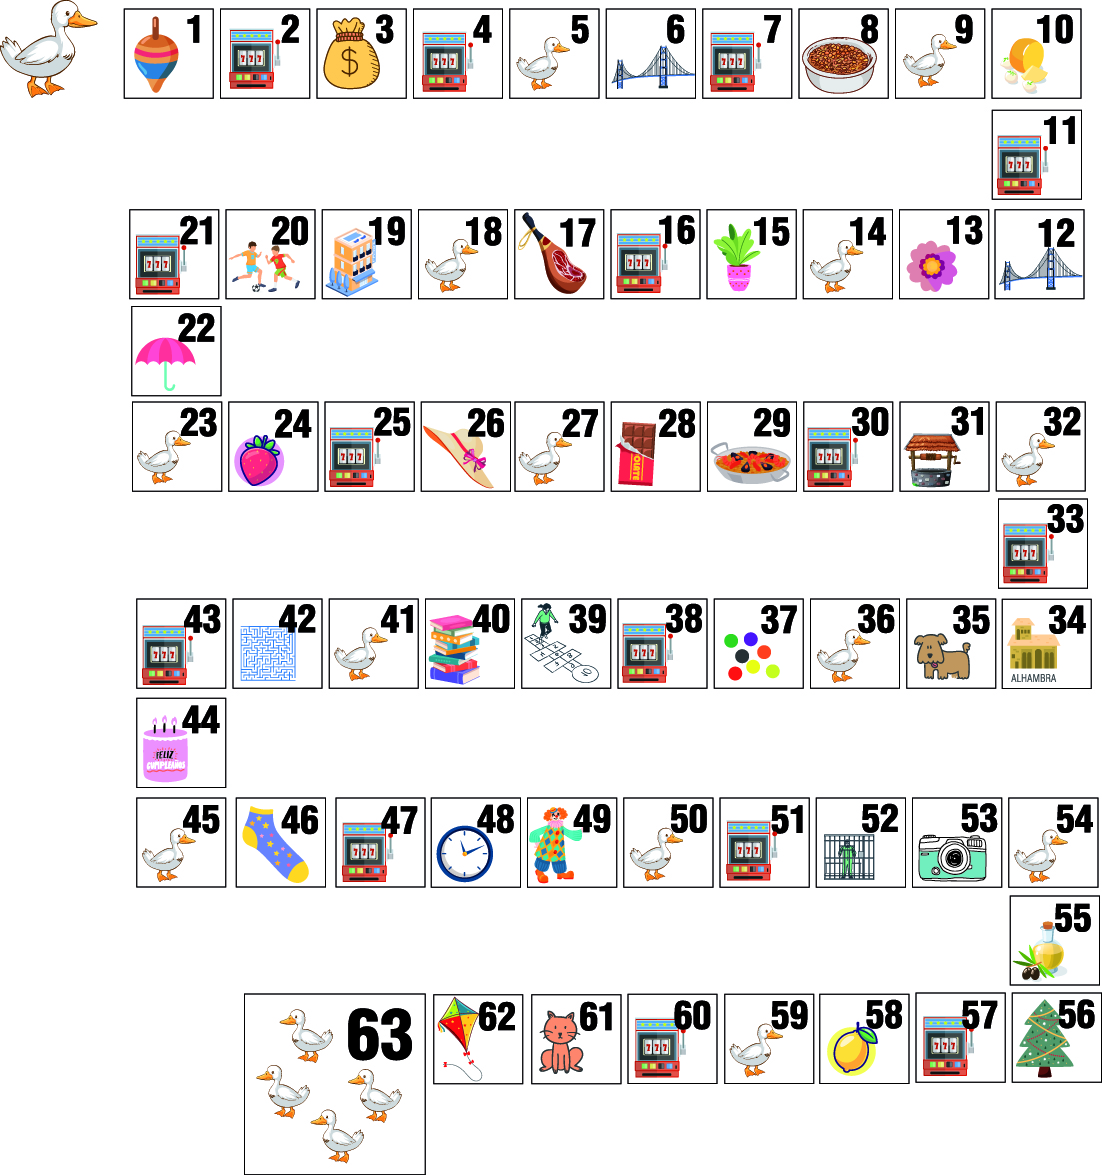
\includegraphics[width=0.98\textwidth]{imgs/tablero-oca.jpg}
	\caption{Tablero de la oca}
	\label{fig:tablero-oca}
\end{figure}
 
La distribución de las casillas es la siguiente: 18 especiales tomadas del juego tradicional (oca, puente, laberinto, pozo, cárcel y hotel), 15 de tipo minijuego y 30 normales. Por tanto, las probabilidades redondeadas a la centésima de caer en cada una son 28,57\%, 23,81\% y 47,62\%, respectivamente. 

\subsubsection{Bocetos y mockups}

\begin{figure}[H]
    \centering
    
\includegraphics[width=0.6\textwidth]{imgs/boceto-bienvenida.JPG}
    \caption{Boceto de la pantalla de inicio de la skill (\href{https://www.lucidchart.com/pages/es}{Lucidchart})}
    \label{fig:boceto-bienvenida}
\end{figure}

\begin{figure}[H]
    \centering
    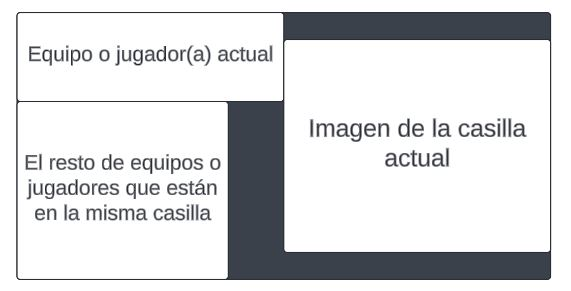
\includegraphics[width=0.6\textwidth]{imgs/boceto-casilla.JPG}
    \caption{Boceto de la pantalla de turno de jugador (\href{https://www.lucidchart.com/pages/es}{Lucidchart})}
    \label{fig:boceto-casilla}
\end{figure}

\subsubsection{Diagrama de flujo entre pantallas}


\subsubsection{Cuestiones de estética, usabilidad y accesibilidad}

Para el estudio de las variables relevantes a la ergonomía del juego, se ha seguido la metodología utilizada en un juego digital para adultos mayores llamado \textit{Solitaire Quiz}. Este está inspirado en el \textit{Solitario}, un juego de cartas tradicional, y a diferencia del original, incluye contenidos didácticos en forma de pequeños cuestionarios. \parencite{diseño2017}.

\begin{table}[H]
	\centering
	\begin{tabular}{|c|p{6cm}|}
		\hline
		\textbf{Categoría} & \textbf{Variables}\\
		\hline
		\multirow{3}{*}{Diseño del juego} & - Desafío \\
		& - Contenido del aprendizaje \\
		& - Retroalimentación \\
		\hline
		\multirow{4}{*}{Usabilidad} & - Ambiente externo al juego \\
		& - Ambiente interno al juego \\
		& - Elementos visuales \\
		& - Dispositivos \\
		\hline
		\multirow{3}{*}{Legibilidad} & - Texto \\
		& - Imágenes \\
		& - Audio \\
		\hline
	\end{tabular}
	\caption{Dimensiones y variables de la ergonomía de la app}
	\label{tab:usabilidad}
\end{table}

%http://agora.edu.es/servlet/articulo?codigo=7894537


%https://www.edutec.es/revista/index.php/edutec-e/article/view/1021